%\documentclass[a4paper]{memoir}
\documentclass[a4paper, 12pt]{report}
\usepackage[top=2.5cm, bottom=2.5cm, left=3cm, right=3cm]{geometry}
%\documentclass[a4paper]{article}
\usepackage[utf8]{inputenc}
\usepackage[english]{babel}
\usepackage{hyperref}
\usepackage{minted}
\usepackage{amsmath}
\usepackage{graphicx}
\usepackage{xcolor}
\definecolor{LightGray}{gray}{0.95}
\usepackage{listings}
%\usepackage{color}
\usepackage{float}
\usepackage[justification=centering]{caption}
\usepackage{caption}
\usepackage{verbatim}
\usepackage{xifthen}
\usepackage{tikz}
\usepackage{lscape} 
\usepackage{pdflscape}
\usepackage{diagbox}
\usepackage{multirow}
\usepackage{algorithm}
\usepackage{algorithmic}
\let\oldv\verbatim
\let\oldendv\endverbatim
\usepackage[square,sort,comma,numbers]{natbib}
\usepackage[OLDMEK, 30]{masterfrontpage}
\usepackage[edges]{forest}
\definecolor{folderbg}{RGB}{124,166,198}
\definecolor{folderborder}{RGB}{110,144,169}
\newlength\Size
\setlength\Size{4pt}
\tikzset{%
  folder/.pic={%
    \filldraw [draw=folderborder, top color=folderbg!50, bottom color=folderbg] (-1.05*\Size,0.2\Size+5pt) rectangle ++(.75*\Size,-0.2\Size-5pt);
    \filldraw [draw=folderborder, top color=folderbg!50, bottom color=folderbg] (-1.15*\Size,-\Size) rectangle (1.15*\Size,\Size);
  },
  file/.pic={%
    \filldraw [draw=folderborder, top color=folderbg!5, bottom color=folderbg!10] (-\Size,.4*\Size+5pt) coordinate (a) |- (\Size,-1.2*\Size) coordinate (b) -- ++(0,1.6*\Size) coordinate (c) -- ++(-5pt,5pt) coordinate (d) -- cycle (d) |- (c) ;
  },
}
\usetikzlibrary{calc}
%\usetikzlibrary{decorations.pathmorphing}
\usetikzlibrary{%
    decorations.pathreplacing,%
    decorations.pathmorphing%
}
\forestset{%
  declare autowrapped toks={pic me}{},
  pic dir tree/.style={%
    for tree={%
      folder,
      font=\ttfamily,
      grow'=0,
    },
    before typesetting nodes={%
      for tree={%
        edge label+/.option={pic me},
      },
    },
  },
  pic me set/.code n args=2{%
    \forestset{%
      #1/.style={%
        inner xsep=2\Size,
        pic me={pic {#2}},
      }
    }
  },
  pic me set={directory}{folder},
  pic me set={file}{file},
}

\title{NEED A TITLE!!!}
\author{Peter Even Killingstad}
\pagenumbering{roman} % Start roman numbering
\begin{document}
\masterfrontpage
\begin{abstract}
 write a short abstract here
\end{abstract}
\tableofcontents

\chapter{Introduction}
\pagenumbering{arabic} % Switch to normal numbers
\chapter{Theory: Governing equations, Turbulence, and Numerical methods.}
\section{Governing equations}
The study of viscous flow reaches back to acient times. Humans figured out, with clever intuision, trial and error, the importance of viscous friction. Long before any real theoretical understanding of fluid flow, streamlined weapons and boats have been made to overcome the effects of viscosity. In more recent years the understanding has taken huge leaps. Today we have tools to master viscous flow with the help from theory. The fundamental equation describing viscous flow is called Navier-Stokes equation\cite{White}. With the following assumptions: incompressible, newtonian fluids. Density and viscosity may be different, but for one fluid it is constant. This gives the following equations:
\begin{eqnarray}
\label{eqn:continuity}
\nabla \cdot \mathbf{u} &=& 0 \\ 
\label{eqn:momentum}
\frac{\partial \rho \mathbf{u}}{\partial t} + \nabla \cdot \big(\rho \mathbf{u} \mathbf{u}\big) &=& \nabla p + \mu \nabla^2 \mathbf{u} + \rho\mathbf{g} + \mathbf{f}_{st} 
\end{eqnarray}
where (\ref{eqn:continuity}) is the conservation of mass and (\ref{eqn:momentum}) is the conservation of momentum. $\mathbf{u}$ is the velocity, $p$ is the pressure, density is given by $\rho(\mathbf{x},t)$, the dynamic viscosity is given by $\mu$, $\mathbf{g}$ and $\mathbf{f}_{st}$ is the gravity and surface tension respectively. There are four independent variables, the spatial $x, y$ and $z$ coordinates, and the time $t$.\\
\\
The equations are a set of coupled differential equations. In practice, these equations are to difficult to solve analytically, but solutions for some simple geometries and boundary conditions can be found. More complex cases, as almost all flows of engineering significance, needs to bee approximated with numerical techniques. Computational fliud dynamics has become the most viable tool to represent the complex Navier-Stokes equations. Some CFD models will be briefly introduced later in this chapter.\\
\\
Using Navier stokes (\ref{eqn:continuity} and \ref{eqn:momentum}), the goal would be to investigate the forces in most industrial and academic applications. Finding solutions to the equations, either analytical or approximations, makes it possible to calculate the force vector by using:
\begin{equation}
\mathbf{F} = \int_{surface} \Big(\nu\big(\nabla \mathbf{u} + (\nabla \mathbf{u})^T\big) - p \mathbf{I}\Big) \cdot \mathbf{n} ds.
\label{eqn:forceVector}
\end{equation}
$\mathbf{n}$ is the unit vecctor normal to the surface, $\mathbf {I}$ is the unit matrix and $\nu$ is the kinematic viscosity. \\
\\
Having obtained the force vector, it is usual to quantify the the drag force or resistance by introducing the drag coefficient, a dimensionless quantity given by
\begin{equation}
C_d = \frac{F_d}{\frac{1}{2}\rho S u^2}.
\label{eqn:dragCoeff}
\end{equation}
Here $F_d$ is the drag force, $\rho$ is density, $u$ is the freestream velocity and $S$ is the surface area. \\
\\
Viscous flows can be divided into several regimes, and the primary controlling parameter is the dimensionless Reynolds number\cite{White}.
\begin{equation}
Re = \frac{u_0l_0}{\nu}
\label{eqn:ReynoldsNumber}
\end{equation}
where $u$ is a velocity scale, $l_0$ is a characteristic geometric size and $\nu$ is the kinematic viscosity. $Re$ represents the ratio of inertial forces to viscous forces within a fluid flow. Fluid properties can cause dramatic changes to the flow patterns. It is usual to divide flows into three distinct regimes.
\begin{itemize}
	\item Low Re flow: \\ Viscous forces dominates and the flow is smooth or laminar regime.
	\item Intermidieate Re flow: \\ Flow is in a transitional region where it is partly fluctuating and partly laminar regime.
	\item High Re flow: \\ Inertial forces dominates and the flow is fluctuating or in a turbulent regime.
\end{itemize} 
Objects advancing through fluids such as water generate free surface waves. At the same time, if an object is advancing through stratified fluids, it generates internal waves. While free surface waves depend on the Froude number: 
\begin{equation}
Fr = \frac{U_0}{\sqrt{gL_0}},
\label{eqn:FroudeNumber}
\end{equation} 
internal waves depends on the densimetric Froude number:
\begin{equation}
Fr_h = \frac{U_0}{c^*}.
\label{eqn:densimetricFroudeNumber}
\end{equation}
$U_0$ is the ship speed, $g$ is gravity and $L_0$ is the ship length at water level. $c^*$ represents the celerity of the longest internal waves. For an infinitely deep denser fluid, $c^*$ is given as:
\begin{equation}
c^* = \sqrt{gh\frac{\Delta \rho}{\rho_0}}
\label{eqn:celerityWaves}
\end{equation} 
where h is the distance from the free surface to the pycnocline, $\Delta \rho$ is the difference beetwen the density of the stratified fluid.
\section{Turbulence}
\subsection{Physical concepts of turbulence}
Turbulence is the phenomenon where a fluid flow appears to be chaotic and random. Unlike laminar flow, where the fluid flows in an orderly fashion, turbulent flow is rapidly fluctuating in all spatial dimensions. Structures of the flow is varying from large scales comparable to the dimensions of the physical boundaries to small scales.\\
\\
The main characteristics of turbulence is the transfer of energy from larger spatial scales into smaller, happening in a three dimensional space and time(\textcolor{red}{need reference}).\\
\\
 To discuss the main characteristics of turbulence, a usefull concept is that of an "eddy". An eddy can be thought of as typical turbulence pattern of small- and large- scales all co-existing in the same fluid. The eddies consists of vortexes intertwined in a chaotic manner, beeing streched by the mean flow and pulled in random directions by one another(\textcolor{red}{need reference}). This mechanism ultimately leads to braking of the eddies into smaller ones, leading to an "energy cascade"(\textcolor{red}{need reference}).\\
\\
The kinetic energy of the mean flow is extracted by the largest scale eddies. Energy from the largest eddies is further extracted to smaller scales, and the kinetic energy is finally dissipated into thermal energy by the small scale eddies(\textcolor{red}{need reference}).\\
\\
The turbulent kinetic energy is defined by the units $\sim [m^2/s^2] \sim u_0^2$. As turbulence is dissipative, the dissipation rate has the units $[m^2/s^3]$. The dissipation rate of kinetic energy scales as $\epsilon \propto u_0^3/l_0$ \cite{Turbulence}, where $u_0$ and $l_0$ is the characteristic velocity and length of the flow.\\
\\
The dissipation rate of kinetic energy is one of the most important results of turbulence theory, and is reffered to as the Kolmogorov relation \cite{Turbulence}. A turbulent eddy with kinetic energy $u_0^2$ either looses its energy or breaks up into smaller eddies in one time scale or period $T \sim l_0/u_0$.\\
\\
As Reynolds number is very large for turbulent flow, i.e $\frac{u_0l_0}{\nu} \gg 1$, the large scale eddies is independent of the viscosity. To see how viscosity is effecting the turbulent flow, "Kolmogorov micro-scales" can be constructed. Using kinematic viscosity $\nu$ and the dissipation rate $\epsilon$, small scale velocity, length and time can be written out as:
\begin{eqnarray}
\label{eqn:microLength}
\eta &=& \big(\frac{\nu^3}{\epsilon}\big)^{1/4}, \\
\label{eqn:microVelocity}
v &=& \big(\nu\epsilon\big)^{1/4}, \\
\label{eqn:microTime}
\tau &=& \big(\frac{\nu}{\epsilon}\big)^{1/2}, 
\end{eqnarray}  
where  $\eta$ is the micro length-scale, $v$ is the velocity and $\tau$ is the time scale. Reynolds number in the "micro-scale" is given by $\frac{v\eta}{\nu} = 1$, hence the viscosity is of big importance at theese scales. We have that the "micro-scale" eddies is dominated by friction, and small-scale turbulence is almost independent of large scale turbulence for large enough reynolds number.

\subsection{Computer modelling of turbulence}
The modelling of turbulent fluid flows and the Navier-Stokes equations has seen huge advancements as computer speed increases. The number of applications of fluid flow predictions has grown and computerized analysis has become a crucial part in the field of fliud mechanics.\\
\\
There are three main methods for numerically solving Navier-Stokes equations:
\begin{itemize}
	\item Reynolds Averaged Navier Stokes(RANS)
	\item  Large Eddy Simulations(LES)
	\item  Direct Numerical Simulations(DNS)
\end{itemize}
LES and DNS is introduced rather briefly, while RANS will be introduced in a litle bit more detail.
\subsubsection{RANS}
For many enginering purposes, the focus is on the mean effect of turbulence, and it is unecessary to resolve the details on all scales.\\
\\
A key part of RANS is investigating the effects of fluctuations on the mean flow using Reynolds de-composition. The velocity and pressure is decomposed as:
\begin{eqnarray}
\label{eqn:ReynoldsDecompU}
\mathbf{u} &=& \mathbf{U} + \mathbf{u'} \\
\label{eqn:ReynoldsDecompP}
p &=& P + p',
\end{eqnarray}
where $\mathbf{u}$ is the instantaneous flow field, $\mathbf{U}$ is the mean flow field and $\mathbf{u'}$ is the fluctuating part. The same goes for the pressure, where P is mean and p' is the fluctuating part.\\
\\
Substituting the de-composed velocity and pressure (\ref{eqn:ReynoldsDecompU}, \ref{eqn:ReynoldsDecompP}) into Navier-Stokes equations (\ref{eqn:continuity}, \ref{eqn:momentum}) and taking the time-mean, the following continuity and momentum equations using suffix notation is derived:
\begin{eqnarray}
\label{eqn:RANScontinuity}
\frac{\partial U_i}{\partial x_j}  &=& 0 \\
\label{eqn:RANSmomentum}
\frac{\partial U_i}{\partial t} +  \frac{\partial}{\partial x_j}(U_i U_j) &=& -\frac{1}{\rho} \frac{\partial P}{\partial x_i} + \nu \frac{\partial ^2 U_i}{\partial x_j \partial x_j} - \frac{\partial}{\partial x_j} (\overline {u_i' u_j'}).
\end{eqnarray}
Here $U_i$ is the mean velocity, P is the mean pressure and $\overline{u_i'}$ is the mean fluctuating velocity.\\
\\
In the momentum equation (\ref{eqn:RANSmomentum}), the new term $\frac{\partial }{\partial x_j}(\overline{u_i'u_j'})$ is derivative of the Reynolds stress-tensor \citep{UNIK4900}. It appears from the convective part $ \mathbf{u} \cdot \nabla \mathbf{u}$ of Navier-Stokes equations (\ref{eqn:momentum}), and is not really stresses. The physical meaning of the term is the averaged effect of turbulent advection on the mean flow field \cite{UNIK4900}.\\
\\
With the new term, the RANS equations is unclosed, with 6 more unknowns appearing from the Reynolds stress-tensor. The four equations has in total 10 unknowns (pressure, three velocity components and six "stresses"). In order to close the problem, enough equations must be found to solve for all the unknowns. In many models, such as one-equation and two-equation models (see \citep{Wilcox} chapter 4), the Boussinesq eddy-viscosity approximation \citep{CFD} is assumed to be valid. The Reynolds stresses are modelled as follows:
\begin{eqnarray}
\label{eqn:bossinesq}
\tau_{ij} = \overline{u_i'u_j'} = \frac{2}{3}k\delta_{ij} - \nu_t\big(\frac{\partial U_i}{\partial x_j} + \frac{\partial U_j}{\partial x_i}\big)\\
\label{eqn:TurbKineticEnergy}
k = \frac{1}{2}\overline{u_i' u_i'} = \frac{1}{2}\big(\overline{u_1^{'2}} + \overline{u_2^{'2}} + \overline{u_3^{'2}} \big)
\end{eqnarray}
where $k$ is the turbulent kinetic energy per unit mass, $\nu_t$ is the turbulent or eddy viscosity and $\delta_{ij}$ is the Kronecker  delta.\\
\\
Substituting the Boussinesq eddy-viscosity approximation (\ref{eqn:bossinesq}) into the RANS momentum equation (\ref{eqn:RANSmomentum}) leads to:
\begin{equation}
\frac{\partial U_i}{\partial t} +  \frac{\partial}{\partial x_j}(U_i U_j) = -\frac{1}{\rho} \frac{\partial P'}{\partial x_i} +  \frac{\partial}{\partial x_j}\Big[ \big(\nu + \nu_t\big) \frac{\partial U_i}{\partial x_j}\Big].
\end{equation}
where $P' = \big(P + \frac{2k}{3}\delta_{ij} \big)$ called the modified pressure\cite{Pope}, often used in CFD.\\
\\
To complete the closure of the RANS equations, the eddy viscosity term $\nu_t$ needs to be modelled. Dimensional analysis dictates that $\nu_t$ needs to be proportinal to product of a characteristic velocity and a characteristic length scale \cite{Wilcox,AppliedMathematicalModelling}. The difference in models such as the one-equation and two - equation models is the way to calculate the scales. 


\subsubsection{LES}
While RANS has the main focus on the mean flow, LES is resolving large scale turbulence. While the effects of large eddies on the flow is resolved, the effect of the small scale eddies is included by a sub-grid scale models \cite{CFD}. \\
\\
In LES modeling, a spatial filter is used to separate small sclaes from large scales. The method is started off with a filtering function and a "cutoff" witdh, where all scales greater than the "cutoff" width is resolved. \\
\\
A filtering operation  of the filter function function is done in the following manner \cite{CFD}:
\begin{equation}
\overline{\phi}(\mathbf{x}, t) = \int_{-\infty}^{\infty}\int_{-\infty}^{\infty}\int_{-\infty}^{\infty} G(\mathbf{x}, \mathbf{x'} \Delta)\phi(\mathbf{x'},t)dx_1'dx_2'dx_3',
\label{eqn:filteringOperation}
\end{equation}
where $G(\mathbf{x}, \mathbf{x'} \Delta)$ is the filtering function, $\overline{\phi}(\mathbf{x}, t)$ is the filtered function, $\phi(\mathbf{x'},t)$ is the original unfiltered function and $\Delta$ is the "cutoff" witdh. The overbar indicates spatial filtering and not time averaging as with RANS.\\
\\
Filtering the Navier-stokes equations (\ref{eqn:continuity} and \ref{eqn:momentum}) gives the LES continuity and momentum equations as follows:
\begin{eqnarray}
\label{eqn:LEScontinuity}
\frac{\partial \overline{u}_i}{\partial x_j} &=&0\\
\label{eqn:LESmomentum}
\frac{\partial \overline{u}_i}{\partial t} +  \frac{\partial \overline{u}_i \overline{u}_j}{\partial x_j} &=& -\frac{1}{\rho} \frac{\partial \overline{p}}{\partial x_i} + \nu \frac{\partial ^2 \overline{u}_i}{\partial x_j \partial x_j} - \frac{\partial \tau_{ij}}{\partial x_j}.
\end{eqnarray}
Here the overline denotes filtered flow variable, and $\tau_{ij}$ is the sub-grid scale stresses. The sub-grid scale stresses are part of the unresolved sub-grid scales. \\
\\
For further introduction of the LES model, Books such as \cite{CFD} and \cite{LESTurbulence} and papers such as \cite{AppliedMathematicalModelling} is recomended. 
\subsubsection{DNS}
DNS involves numerical solution of the full Navier-Stokes equations. The method resolves all scales, including the kolmogorov scales (\ref{eqn:microLength}, \ref{eqn:microTime} and \ref{eqn:microVelocity}). It takes the closed form of the four equations and four unknowns and solves it on a sufficiently fine mesh and small enough time step. For flows with small enough Reynolds number (\ref{eqn:ReynoldsNumber}), DNS can serve as a benchmark for the other turbulence models \citep{AppliedMathematicalModelling}.\\
\\
Using "Kolmogorov's micro- scales" (\ref{eqn:microLength} and \ref{eqn:microTime}), ratio's of the largest and smallest scales can be obtained. The ratio of the largest and the smallest scales are proportional to  $Re^{3/4}$ and the ratio of the largest and smallest time scale is proportional to $Re^{1/2}$. $Re = 10^4$ requires a spatial resolution of $\mathcal{O}(10^3)$ in each direction, and the simulation must run for atleast $100$ time steps. Computing meshes with $10^9$ grid points with $100$ time steps is very demanding, even with a modest Reynolds number. Computing industrial flows with higher Reynolds number is impossible with current technology \cite{CFD, AppliedMathematicalModelling}.

\section{Volume of fluid}
When there is multiple fluids in a computation, there is need for an interface tracking or interface capturing. To handle multiple-fluid interactions, the volume of fluid method used.\\
\\
For each fluid component, a volume fraction is introduced. If $V$ is a volume of a cell in a computaional domain, and $\alpha(\mathbf{x}, t)$ is the volume fraction, the volume fraction for two fluids is defined as \citep{VOF2}
\begin{equation}
\alpha(\mathbf{x},t) = \left\{
        \begin{array}{ll}
            1, & \quad \mathbf{x} \in \Omega_l \\
            0, & \quad else
        \end{array}
    \right.
\label{eqn:volumeFraction}    
\end{equation}
where $\Omega_l$ is the part of the domain covered by one fliud $l$.\\
\\
On each grid cell, the integral of the color function is approximated. The discrete volume fraction is written as \citep{VOF2}
\begin{equation}
\alpha_i = \frac{1}{V} \int_{V} \alpha(\mathbf{x},t) dV
\end{equation}
where the subscript $i$ denotes the $i$'th fluid in a system.\\
\\
For miscible fluids the volume fractions are governed by the advection-diffusion equation given as \citep{VOF1}
\begin{equation}
\frac{\partial \alpha_i}{\partial t} + \nabla \cdot (\alpha \mathbf{u}) = D\nabla^2 \alpha,
\label{eqn:alphadiffusionEquation}
\end{equation} 
Where D denotes diffusivity between miscible fluids. The following constraint must be satisfied due to mass conservation:
\begin{equation}
\Sigma_{i=1}^n \alpha_i= 1
\label{eqn:alphaConstraint} 
\end{equation}
Desity and viscosity are defined as:
\begin{eqnarray}
\label{eqn:alphaRhodiffusion}
\rho = \Sigma_i \rho_i \alpha_i \\
\label{eqn:alphaMudiffusion}
\mu = \Sigma_i \mu_i \alpha_i
\end{eqnarray}

\section{Numerical discretization}
Numerical discretization is the prosses of transferring differential equations, such as the Navier- Stokes equations (\ref{eqn:continuity} and \ref{eqn:momentum}), into descrete counterparts.
A discretization method is needed in order to evaluate the equations on computers. \\
\\
There are three discretisation methods generally used when approximating equations. Finite difference method, finite element method and finite volume method.\\
\\
As in most commercial well-established CFD codes, this thesis is using the finite volume method. Fvm is one of the most versitaile discretization techniques used in cfd \cite{CFD}.\\
\\
An outline for the disctretization procedure can be presented with the following steps:
\begin{itemize}
\item Integration of the governing equations of fluid flow all over the finite control volumes of the domain.
\item Conversion of the resulting integral equations into a system of algebraic equations.
\end{itemize}
A domain is divided into a number of control volumes where the varable of interest is located in the centeroid of the control volume.

\chapter{OpenFOAM}
All computanial fluid dynamis is structured around numerical algorithms that tackles fliud flow problems. Classical solvers are implemented in well-established CFD codes such as CFX/ANSYS, FLUENT and OpenFOAM. The software used in this thesis is OpenFOAM.\\
\\   
As in all well-established CFD codes, the work flow consists of three main elements:
\begin{itemize}
\item pre-processor
\item solver
\item post-processor
\end{itemize}
Pre-processing consists of input of a flow problem, in order to make it well-defined before the solving process begins.\\
\\
The solver is solving the flow problem, by implemented numerical methods and algorithms suitable for the specific problem. \\
\\
Post-processing consists of verification and validation of the solutions given by the solver. It essential to investigate data output and visualize. The complexity of fluid flows demands thurough investigation by e.g. comparing with existing experiments, either numerical or experimental.\\
\\
\section{Introduction to OpenFoam}
This paper is using the free, open sorce software OpenFOAM (Field Operation and Manipulation). It is a C$++$ library of source code for solvers and utilities.\\
\\
Figure \ref{fig:caseStructure} illustrates an initial state of an OpenFOAM case. Three directories are located in the case folder: 0, constant and system.\\
\\
The 0 directory contains files for the different parameters essential for the problem. Each file defines initial values and boundary conditions for the numerical experiment.\\
\\
The \textit{constant} directory contains, as the name suggests, all the constants of the case. Constant variables such as gravitation \textit{g}, \textit{transportProperties} as density and viscosity and \textit{turbulenceProperties} are defined in separate files. The subdirectory \textit{polyMesh} contains the mesh geometry.\\
\\
The \textit{system} directory contains information about meshing of the numerical experiment, how to discretize and solve the equations. The file controlDict controls ehich solver is used, timecontrols and data output controls. As the names suggests, \textit{fvSchemes} and \textit{fvSolution} contains information about discretization schemes and solution algorithms respectively. 
\begin{figure}[H]
\centering
\begin{forest}
  pic dir tree,
  where level=0{}{% folder icons by default; override using file for file icons
    directory,
  },
  [caseDir
    [0
      [u, file]
      [p\_rgh, file]
      [k, file]
      [nut, file]
      [omega, file]
      [alpha.water, file]
    ]
    [constant
      [polyMesh]
      [g, file]
      [transportProperties, file]
      [turbulenceProperties, file]
    ]
    [system
      [blockMeshDict, file]
      [controlDict, file]
      [fvSchemes, file]
      [fvSolution, file]
      [setFields, file]
    ]
  ]
\end{forest}
  \caption{Example of case directory structure in openFOAM.}
  \label{fig:caseStructure}
\end{figure}


\section{TwoLiquidMixingFoam}
OpenFOAM has solvers for a wide range of applications. Many multiphase solvers can be found, both miscible and immiscible. This thesis is using the incompressible multiphase solver twoLiquidMixingFoam, where the liquids are miscible.\\
\\
Three equations are beeing solved. The first equation is the alpha diffusion equation, given by:
\begin{equation}
\frac{\partial \alpha_1}{\partial t} + \nabla \cdot (\rho \mathbf{U} \alpha_1) = \nabla \cdot \Big(\big(D + \frac{1}{S_C} D_t \big)\nabla \alpha_1 \Big) 
\label{eqn:alphaEqTLMF}
\end{equation}
where
\begin{itemize}
	\item $\alpha$ is the volume fraction.	
	\item $\rho = \alpha_1 \rho_1 + \alpha_2 \rho_2$.
	\item D is the molecular diffusivity.
	\item $D_t$ is the molecular diffusivity due to turbulence.
	\item $s_c$ is the Schmidt number, given as $\mu / (\rho D)$.
\end{itemize}
The continuity and momentum equation is given, respectively, as: 
\begin{eqnarray}
\label{eqn:continuityTLMF}
\nabla \cdot \mathbf{U} &=& 0 \\
\label{eqn:momentumTLMF}
\frac{\partial \rho \mathbf{U}}{\partial t} + \nabla \cdot(\rho \mathbf{U} \mathbf{U}) &=& - \nabla (p\_rgh) - gh\nabla \rho + \nabla \cdot (\rho \boldsymbol{\tau})
\end{eqnarray}
where 
\begin{itemize}
	\item $\boldsymbol{\tau} = -\frac{2}{3}\overline{\mu_{eff}}\nabla \cdot \mathbf{U} \mathbf{I} + \overline{\mu_{eff}}\nabla \mathbf{U} + \overline{\mu_{eff}}\big(\nabla \mathbf{U}\big)^T$.
	\item $\overline{\mu_{eff}} = \alpha_1 (\mu_{eff})_1 + \alpha_2 (\mu_{eff})_2$.
	\item $(\mu_{eff})_i = (\mu - \mu_t)_i$. Subscript $i$ denotes either fluid 1 or 2.
\end{itemize}
The term $\nabla(p\_rgh)$ and $gh \nabla \rho$ is obtained by using $P = p\_rgh + \rho gh$. The Solver is using the Boussinesq eddy-viscosity approximation (\ref{eqn:bossinesq}), and $p$ is the modified pressure and containes the kinetic energy per unit mass $\frac{2}{3}k\delta_{ij}$. 

\section{Solution algorithms}
There is three different pressure correction algorithms implemented in OpenFOAM, namely SIMPLE, PISO and PIMPLE. SIMPLE is a steady state algorithm, PISO is a transient algorithm and PIMPLE is a semi transient algorithm.\\
\\
\begin{algorithm}
\caption{Calculate $y = x^n$}
\begin{algorithmic}
\REQUIRE $n \geq 0 \vee x \neq 0$
\ENSURE $y = x^n$
\STATE $y \leftarrow 1$
\IF{$n < 0$}
\STATE $X \leftarrow 1 / x$
\STATE $N \leftarrow -n$
\ELSE
\STATE $X \leftarrow x$
\STATE $N \leftarrow n$
\ENDIF
\WHILE{$N \neq 0$}
\IF{$N$ is even}
\STATE $X \leftarrow X \times X$
\STATE $N \leftarrow N / 2$
\ELSE[$N$ is odd]
\STATE $y \leftarrow y \times X$
\STATE $N \leftarrow N - 1$
\ENDIF
\ENDWHILE
\end{algorithmic}
\end{algorithm}

\chapter{Simulation Design}
Wether an numerical experiment is succesfull depends largely on the pre-processing. A computational domain has to be made well suited to handle the flow problem. Many factors has to be considered in order to have a good numerical experiment, with mesh quality and and boundary conditions as the key factors.
\section{Simulation geometry}
The geometry of the numerical experiment is dependent on computational demands. Ideally the geometry of the domain would include the entire barge and a farfield consisting of air, fresh- and salt-water. A domain including all aspects of the fluid problem would bee much more suitable as the case would bee more physical.\\
\\
With a three dimensional problem such as the "dead-water" phenomenon, the computational costs constrains the experiment to some parts of the flow problem. This and the scope of this thesis, which is limited to five months, makes it necessary to make comprimise between physics and assumptions. The experiment becomes less physical, but the idea is to isolate certain aspects of the problem to investigate, namely the effects of the internal wave.\\
\\
The geometry of the computational domain consists of a barge surface and a farfield. Farfield includes inlet, outlet, atmosphere, bottom, front and back in order to have a closed domain. Only the draft of the barge is included, making the top of the domain located at the free-surface.\\
\\
Figure \ref{fig:domain} is showing simulation gemoetry with patches atmosphere, front, inlet and outlet included. The Barge is colored red. The dimensions of the barge is taken from \cite{Gou} and $0.6$ m long (x-dir), $0.45$ m wide (y-dir) and $0.35$ m wide (z-dir).  The geometry used in the numerical experiment is using a symmetry plane in y-direction, halving the computational domain. It further only includes what is below the free surface i.e. the draft of the barge. The dimensions of the barge is therefore $0.6$m long, $0.225$m wide and draft is $0.1$m.\\
\\
Farfield boundaries are located sufficiently far away to minimize effects of the boundaries on the solution. international Towing Tank Conference has a practical guidelines for ship CFD applications which states that inlet, outlet and "exterior boundary" should be located $1-2$ $\times$ length at draft \cite{ITTC}. This experiment is not modelling the free surface as it is a boundary. It does however modell an internal wave and in combination with highly unstreamlined draft geometry, the resulting farfield  dimensons are:
\begin{itemize}
\item inlet located $10.0$ m upstream in front of barge.
\item outlet located $-15.0$ m downstream of barge.
\item bottom located at $-4.0$ m below barge.
\item back is located $3.0$ m at the width side of barge.
\end{itemize}

\begin{figure}[H]
	\centering
	\includegraphics[width=0.8\textwidth]{/home/peterek/OpenFOAM/PETER-5.0/MT_PK/plots/paraView/MESH/MeshBoundaries.png}
	\caption{Geometry. \\ \textit{Geometry used in the computational experiment. Draft of barge is colored red at $X = 0$ while farfield with patches inlet, outlet, front and atmosphere included.}}
	\label{fig:domain}
\end{figure}

\section{Simulation set-up}
Simulations is done with a constant draft $D = 0.1$ m.  The different experiments is conducted by varying the densimetric Froude number in the range $0.3 \leq Fr_h \leq 1.35$.  The densimetric Froude number is varied by changing speeds at constant pycnocline depths giving $h/D$ $=$ $1$, $1.5$ and $2$.\\
\\
Figure \ref{fig:experiment} is showing a schematic overview of the numerical experiment.\\
\\
The experiments are done with a moving reference frame, rather than having the barge moving, in order to be able to run simulations sufficiently long.\\
\\
The densities of the fluids are set to $997$ kg m$^{-3}$ for fresh water and $1024$ kg m$^{-3}$ for salt water. Kinematic viscosity is set to $\nu = 1.79 \cdot 10^{-6} m^2 s^{-1}$ corresponding to waters at $0^{\circ}$C. The speed  varies as $0.08\leq U \leq 0.22$ corresponding to Reynolds number (\ref{eqn:ReynoldsNumber}) $26815 \leq Re \leq 73743$.\\
\\

\begin{figure}[H]
\centering
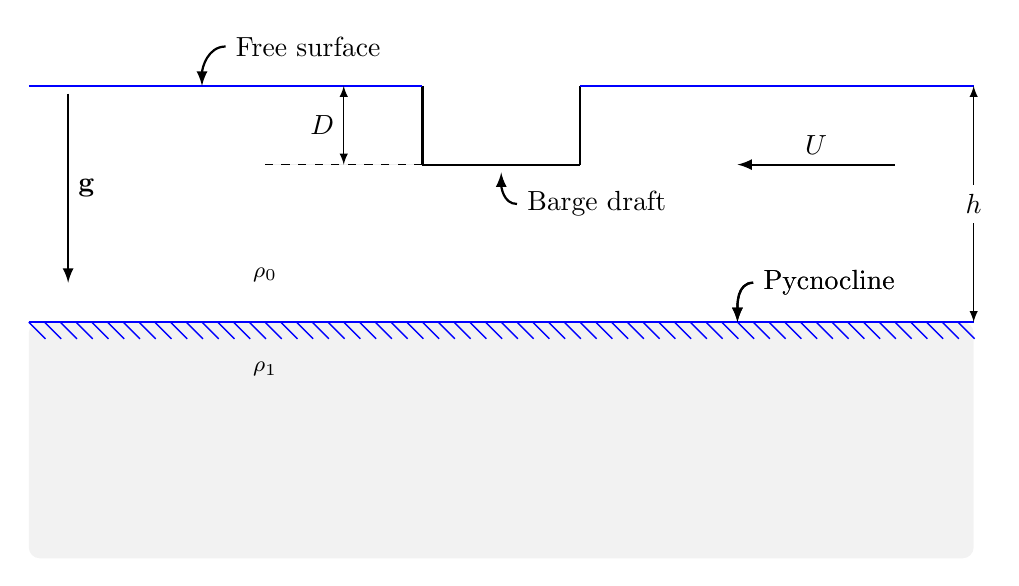
\begin{tikzpicture}[
    media/.style={font={\footnotesize\sffamily}},
    wave/.style={
        decorate,decoration={snake,post length=1.4mm,amplitude=2mm,
        segment length=2mm},thick},
    interface/.style={
        % The border decoration is a path replacing decorator. 
        % For the interface style we want to draw the original path.
        % The postaction option is therefore used to ensure that the
        % border decoration is drawn *after* the original path.
        postaction={draw,decorate,decoration={border,angle=-45,
                    amplitude=0.3cm,segment length=2mm}}},
    dimen/.style={<->,>=latex,thin,
        every rectangle node/.style={fill=white,midway,font=\sffamily}},
    ]
    % Round rectangle
    \fill[gray!10,rounded corners] (-6,-3) rectangle (6,0);
    % Interface
    \draw[blue,line width=.5pt,interface](-6,0)--(6,0);
    % barge
    \draw[thick,black](-1,3)--(-1,2);
    \draw[thick,black](-1,2)--(1,2);
    \draw[thick,black](1,2)--(1,3);
        \draw[-latex,thick](3.2,0.5)node[right]{Pycnocline}
         to[out=180,in=90] (3,0);
    % free surface     
    \draw[thick,blue](-6,3)--(-1,3);
    \draw[thick,blue](1,3)--(6,3);
    % Coordinates system
    %\draw(0,0.15)node[above]{$x$};
    %\draw[<->,line width=1pt] (1,0) node[above]{$y$}-|(0,-1) node[left]{$z$};

    % Media names
    \path[media] (-3,.6)  node {$\rho_0$}
                 (-3,-.6) node {$\rho_1$};
    \draw[dimen] (6,3) -- (6,0) node {$h$};
    \draw [-latex,thick](5,2) -- (3,2)	node [midway,above] {$U$};
    \draw [-latex,thick](-5.5,2.9) -- (-5.5,0.5)	node [midway,right] {$\mathbf{g}$};    
	\draw [fill=gray,dashed] (-1, 2) --(-3, 2); 
	\draw[dimen] (-2,3) -- (-2,2) node [left] {$D$};
    % $x$ axis

    % Interface pointer
    \draw[-latex,thick](3.2,0.5)node[right]{Pycnocline}
         to[out=180,in=90] (3,0);
    % Barge pointer
    \draw[-latex,thick](0.2,1.5)node[right]{Barge draft}
         to[out=180,in=270] (0,1.9);
    % Free surface pointer
    \draw[-latex,thick](-3.5,3.5)node[right]{Free surface}
         to[out=180,in=90] (-3.8,3);         
    % To-paths are really useful for drawing curved lines. The above
    % to path is equal to:
    %
    % \draw[-latex,thick](3.2,0.5)node[right]{$\mathsf{S_{1,2}}$}
    %      ..controls +(180:.2cm) and +(up:0.25cm) .. (3,0);
    % Internally the to path is translated to a similar bezier curve,
    % but the to path syntax hides the complexity from the user. 
\end{tikzpicture}
\caption{Simulation set-up. \\ \textit{Simulations is done by varying speeds $U$ at constant $h/D = 1$, $1.5$ and $2$. Densities $\rho_0$ and $\rho_1$ is that of fresh- and salt-water respectively for stratified fluid simulations. For non-stratified fluid simulations, $\rho_0 = \rho_1$ }}
\label{fig:experiment}
\end{figure}

\section{Boundary and Initial conditions}
Before simulating and solving the numnerical experiment, the momentum and continuity equations (\ref{eqn:momentum} \ref{eqn:continuity}) must have appropriate initial and boundary conditions.\\
\\
Boundary conditions are required component of the mathematical model that directs the motion of the flow. It specifies the fluxes such as mass and momentum into and out of the computational domain.\\
\\
OpenFOAM is representing boundaries as patches consisting of faces, and all inital and and boundary data are assigned to the patches. Table \ref{tbl:boundaries} is showing an overview of all initial and boundary conditions.\\
\\
\subsection{U}
For velocity U, typical dirichlet boundary conditions is a applid at the inlet and on the barge. At the inlet there is \textit{fixedValue}  while a no-slip condition is set at the barge. The no-slip condition is a of a special kind, namely \textit{movingWallVelocity}, which is applied for "moving" walls when it is a moving reference frame.\\
\\
At outlet there is an \textit{outletPhaseMeanVelocity}. This boundary condition adjusts the velocity for the given phase to achieve the specified mean, thus causing the phase-fraction to adjust according to the mass flow rate.\\
\\
\subsubsection{Boundaries for the free surface}
Since the simulation only includes what happens below the water surface, and the main focus of the experiments is the investigation of the internal wave it, has been rather tricky to decide boundaries for the free surface. The free surface waves that is generated should bee of very small wave length and height due to low Froude numbers (\ref{eqn:FroudeNumber}), as $Fr \leq 0.09 $. An approach has been to apply a Neumann boundary condition of zero gradient at the top. With a zero gradient at the top, the bow of the barge would have been well approximated as the fluid hits the bow and it would allow outflow. At the stern however, the lower pressure would allow inflow. This would have been a good approximation, if the inflow had been consisting of air. The problem is that the inflow at the stern consists of water, causing the interface at the stern to mix and loosing of the stratified water. \\
\\
Another approach as been to use a slip condition, which is a mix of Dirichlet and Neumann condition. The flow would then be allowed to flow freely in x- and y direction, but be set at z-direction. This would not allow for in- and outflow.\\
\\
With the low Froude number and the goal of the invistigation beeing the internal wave, this could have been a good approximation. The \textit{slip} condition caused an numerical artifact at at a point of the bow of the barge where another boundary condition of symmetry was set. The \textit{symmetryPlane} condition at the front of the domain allows outflow, causing a one cell intersecting both boundary conditions having very large velocity.\\
\\
A comprimise has been done, with the top of the domain beeing split into two patches, namely \textit{atmosphere} and \textit{atmosphereFrontOfBarge}. The \textit{atmosphere} patch having a \textit{slip} boundary condition and the \textit{atmosphereFrontOfBarge} having an \textit{inletOutlet} condition. The \textit{inletOutlet} condition is working as a Neumann condition, with the specification of inflow, in case there is any. \\
\\
These boundary conditions has a very engineering approach to them, and is not very physical. But as stated earlier in this repert, the main focus is the effect of the internal wave. With the air excluded completely from the simulations, and the low Froude numbers, the final boundary conditions of the free surface is sufficient with the goal of the experiment.
\subsection{alpha.saltWater}
The phase fraction \textit{alpha.saltWater} is set in the file \textit{setFieldsDict} where the initial state of the fluid is set.\\
\\
As for the boundaries, a fixed value of either $1$ or $0$ is set, where $1$ is salt water and $0$ is fresh water, is set at the inlet. At the outlet, a \textit{variableHightFlowRate} condition is used. It is a phase fraction condition based upon the flow conditions. Values of \textit{alpha.water} is constrained to lay between specified values of upper and lower bounds of $1$ and $0$, i.e.
\begin{itemize}
\item If \textit{alpha.water} > 1:
	\begin{itemize}
	\item apply a fixed value, with a uniform level $1$.
\end{itemize}
\item If $0$ $\leq$ \textit{alpha.saltWater} $\leq$ $1$:
	\begin{itemize}
	\item apply a \textit{zeroGradient} condition.
	\end{itemize}
\item If \textit{alpha.water} < 0:
	\begin{itemize}
	\item apply a fixed value, with a uniform level $0$.
\end{itemize}
\end{itemize}
At the \textit{barge}, a Neumann condition of \textit{zeroGradient} is applied. The same goes for \textit{atmosphere} and \textit{atmosphereFrontOfBarge}.
\subsection{p\_rgh}

\subsection{Turbulence properties k, nut, omega and epsilon}
All of the turbulence properties nut, k, omega and epsilon are set with \textit{zeroGradient} at the top patches \textit{atmosphere} and \textit{atmosphereFrontOfBarge}.\\
\\
At the inlet, Dirichlet boundaries are set as a fixed value, calculated from equations for setting farfield turbulence conditions.\\
\\
Farfield turbulent kinetic energy is set by using:
\begin{equation}
k = \frac{3}{2}(UI)^2,
\label{eqn:turbulentKineticEnergy}
\end{equation}
where U is the freestrem speed and I is the turbulence intensity, usually set below 1\% for cases similar to this experiment. \\
\\
Farfield omega conditions is set by using:
\begin{equation}
\omega = \frac{\sqrt{k}}{C_{\mu}^{1/4}l_t}
\label{eqn:turbulentOmega}
\end{equation}
where $C_{\mu}=0.09$ and $l_t$ is the turbulent length scale, set to $l/100$ where l is the length of the barge.\\
\\
Turbulent dissipation rate epsilon is set by using:
\begin{equation}
\epsilon =  \frac{c_{\mu}^{3/4} k^{3/2}}{l_t}
\label{eqn:turbulentDissipationRate}
\end{equation}
Finally, the turbulent viscosity is set by using:
\begin{equation}
\nu_t = \frac{k}{\omega}
\label{eqn:turbulentViscosityFarfield}
\end{equation}
\subsubsection{Wall functions}
 At the barge, wall functions is applied as boundary conditions for all the turbulence properties. 
\begin{landscape}
	\begin{table}[H]
		\centering
		\begin{tabular}{c|c|c|c|c|c|c|c}
			\multicolumn{2}{c|}{\diagbox{Boundary}{Variable}} & U&p$\_$rgh & alpha.saltWater  & k & omega & nut \\\cline{1-8}
			
			\multirow{2}*{Inlet} & Type & fixedValue & fixedFluxPressure & fixedValue &  fixedValue & fixedValue & fixedValue\\
			&Value & internalField & internalField & internalField &  internalField & internalField &internalField \\\cline{1-8}
			
			\multirow{2}*{Outlet} & Type & O.P.M.V. & zeroGradient & V.H.F.R. &  inletOutlet & inletOutlet & zeroGradient\\
			&Value & internalField & - & internalField &  internalField & internalField &- \\\cline{1-8}
			
			\multirow{2}*{Barge} & Type & M.W.V. & F.F.P. & zeroGradient & kqrW.F. & omegaW.F. & nutUSpaldinW.F.\\
			&Value & (0 0 0) & internalField & - & internalField & internalField &internalField \\\cline{1-8}
			
			\multirow{2}*{atmosphere} & Type & slip & fixedValue & zeroGradient & zeroGradient & zeroGradient & zeroGradient\\
			&Value & - & internalField & - &  - &- &-\\\cline{1-8}
			
			\multirow{2}*{atmosphereFrontOfBarge} & Type & inletOutlet & fixedValue & zeroGradient &  zeroGradient & zeroGradient & zeroGradient\\
			&Value & internalField & internalField & - & - & - &-\\\cline{1-8}
			
			\multirow{2}*{Front} & Type & symmetryPlane & symmetryPlane & symmetryPlane &  symmetryPlane &symmetryPlane & symmetryPlane\\
			&Value & - & -& - & - &- &-\\\cline{1-8}
			
			\multirow{2}*{Back} & Type & symmetryPlane & symmetryPlane & symmetryPlane & symmetryPlane & symmetryPlane & symmetryPlane\\
			&Value & - & - & - & - & -& -\\\cline{1-8}
			
			\multirow{2}*{Bottom} & Type & symmetryPlane & symmetryPlane & symmetryPlane &  symmetryPlane & symmetryPlane & symmetryPlane\\
			&Value & - & - & - & - & -& -\\\cline{1-8}
			
		\end{tabular}
		\caption{Boundary and initial conditions twoLiquidMixing with k-omega SST turbulence model.\\
			O.P.M.V. = OutletPhaseMeanVelocity, V.H.F.R. = variableHightFlowRate, M.W.V. = movingWallVelocity, F.F.P. = fixedFluxPressure,\\ kqrW.F. = kqrWallFunction, omegaW.F. = omegaWallFunction, nutUSpaldingW.F. = nutUSpaldingWallFunction}
		\label{tbl:boundaries}
	\end{table}
\end{landscape}

\section{Mesh and mesh convergence}
Three grids has been systematically refined to evaluate grid convergence. With a grid refinement ratio of $\approx 2$, the resulting course, medium and fine grids have $4.2\times 10^5$, $7.4\times 10^5$ and $1.3\times 10^6$ cells respectively.\\
\\
Two speeds at two different pycnocline depths are used to check for convergence, resulting in  four tests. For each pycnocline depth, two velocities gives  densimetric Froude number corresponding to near-peak drag coefficient and densimetric Froude number close to critical  where drag coefficients changes rapidly as a function of densimetric Froude number.\\
\\ 
\begin{minipage}{.45\textwidth} 
	\begin{figure}[H]
		\centering
		\includegraphics[width=0.99\textwidth]{/home/peterek/OpenFOAM/PETER-5.0/MT_PK/plots/meshSensitivity/U014Interface01.png}
		\caption{$C_d$ as a function of time. \\ \textit{}}
		\label{fig:convTestIf01U01}
	\end{figure}
\end{minipage}\hfill
\vspace{2ex}
\begin{minipage}{.45\textwidth} 
	\begin{figure}[H]
		\centering
		\includegraphics[width=0.99\textwidth]{/home/peterek/OpenFOAM/PETER-5.0/MT_PK/plots/meshSensitivity/U022Interface01.png}
		\caption{$C_d$ as a function of time. \\ \textit{}}
		\label{fig:convTestIf01U022}
	\end{figure}
\end{minipage}\hfill
\vspace{2ex}
\begin{minipage}{.45\textwidth} 
	\begin{figure}[H]
		\centering
		\includegraphics[width=0.99\textwidth]{/home/peterek/OpenFOAM/PETER-5.0/MT_PK/plots/meshSensitivity/U014Interface02.png}
		\caption{$C_d$ as a function of time. \\ \textit{}}
		\label{fig:convTestIf02U016}
	\end{figure}
\end{minipage}\hfill
\vspace{2ex}
\begin{minipage}{.45\textwidth} 
	\begin{figure}[H]
		\centering
		\includegraphics[width=0.99\textwidth]{/home/peterek/OpenFOAM/PETER-5.0/MT_PK/plots/meshSensitivity/U022Interface02.png}
		\caption{$C_d$ as a function of time. \\ \textit{}}
		\label{fig:convTestIf02U022}
	\end{figure}
\end{minipage}\hfill
\vspace{2ex}

\chapter{Analysis and discussion of Results}
\section{internal wave}

\section{Drag}
At critical densimetric froude numbers, the drag increases. The reason for the increase in drag is because we get a crest of the internal wave at the stern of the barge. The crest restricts the passage area and accelerates the flow. This in turn results in a lower pressure in the stern of the ship. We get both a higher friction drag, and the lower pressure for the stratified case increases the pressure drag. In total we get an increase in the stratified case.\\
\\ 
Key points to include:
\begin{itemize}
	\item crest at stern of barge
	\item increase of velocity because of restriction of passage area
	\item results in thinner boundary layer, thus hicgher friction.
	\item also results in decrease of the pressure, such that total drag coefficient increses
\end{itemize}

\begin{figure}[H]
	\centering
	\includegraphics[width=0.8\textwidth]{/home/peterek/OpenFOAM/PETER-5.0/MT_PK/plots/3Dtop/Gou2KOSpaldingRefType2kLowRe.png}
	\caption{Drag force as function of velocity squared. \\ \textit{Resistance in homogeneous fluid with barge draft $=0.1$. Simulations is in good agreement with experimental data obtained on an identical barge done by Gou et. al. \cite{Gou} with a deviance of approximately 20 \%. Resistance is directly proportianal to the square of the towing speed, which means that the drag coefficient is constant. }}
	\label{fig:dragForce}
\end{figure}

\begin{figure}[H]
	\centering
	\includegraphics[width=1\textwidth]{/home/peterek/OpenFOAM/PETER-5.0/MT_PK/plots/3Dtop/Surface.png}
	\caption{Pycnocline as a function of x-position. \\ \textit{Pycnocline (internal wave interface) below the barge as a function of x-position. Pycnocline is initially at $z = 0.2$ for the stratified case. For the non-stratified (single) case, there is a transported passive scalar. As $Fr_h$ increases, wave amplitude increase and it's corresponding x-position is located further back. Location of amplitude has significant effect on flow field as shown in figure \ref{fig:velocityProfileX0} and \ref{fig:velocityProfileX03}. The internal wave restricts the passage area. This in turn effects $C_d$ as shown in figure \ref{fig:Cd}. }}
	\label{fig:eta}
\end{figure}

\begin{figure}[H]
	\centering
	\includegraphics[width=0.8\textwidth]{/home/peterek/OpenFOAM/PETER-5.0/MT_PK/plots/3Dtop/VelocityProfileX0.png}
	\caption{Dimensionless velocity profiles $U_x/U_0$ as function of z-position. \\ \textit{Dimensionlesss velocity profiles $U_x/U_0$ at the stern of barge at $x = 0.0$ m with pycnocline at $ 0.2$. For $Fr_h$ = $0.69$, which has peak $C_d$, there is an increase in velocity and a big velocity gradient. This is causing a lower pressure and smaller boundary layer.}}
	\label{fig:velocityProfileX0}
\end{figure}

\begin{figure}[H]
	\centering
	\includegraphics[width=0.8\textwidth]{/home/peterek/OpenFOAM/PETER-5.0/MT_PK/plots/3Dtop/VelocityProfileX2.png}
	\caption{Dimensionless velocity profiles $U_x/U_0$ as function of z-position. \\ \textit{Dimensionlesss velocity profiles $U_x/U_0$ below barge at $x = 0.3$ m with pycnocline at $ 0.2$. The velocity profile with $Fr_h = 0.35$ has a signifiant increase and a big gradient. The effect on $C_d$ for $Fr_h = 0.35$ is not as significant even though velocity increaces due to the location of the internal wave, shown in figure \ref{fig:eta}.  }}
	\label{fig:velocityProfileX03}
\end{figure}

\begin{minipage}[t]{.45\textwidth}
	\begin{figure}[H]
		\centering
		\includegraphics[width=0.99\textwidth]{/home/peterek/OpenFOAM/PETER-5.0/MT_PK/plots/3Dtop/VelocityProfileX0.png}
		\caption{$C_d$ as a function of time. \\ \textit{Dimensionlesss velocity profiles $U_x/U_0$ at the stern of barge at $x = 0.0$ m with pycnocline at $ 0.2$. For $Fr_h$ = $0.69$, which has peak $C_d$, there is an increase in velocity and a big velocity gradient. This is causing a lower pressure and smaller boundary layer.}}
		\label{fig:convTestIf02U016}
	\end{figure}
\end{minipage}\hfill
\vspace{2ex}
\begin{minipage}[t]{.45\textwidth} 
	\begin{figure}[H]
		\centering
		\includegraphics[width=0.99\textwidth]{/home/peterek/OpenFOAM/PETER-5.0/MT_PK/plots/3Dtop/Surface.png}
		\caption{$C_d$ as a function of time. \\ \textit{Dimensionlesss velocity profiles $U_x/U_0$ below barge at $x = 0.3$ m with pycnocline at $ 0.2$. The velocity profile with $Fr_h = 0.35$ has a signifiant increase and a big gradient. The effect on $C_d$ for $Fr_h = 0.35$ is not as significant even though velocity increaces due to the location of the internal wave, shown in figure \ref{fig:eta}.  }}
		\label{fig:convTestIf02U022}
	\end{figure}
\end{minipage}\hfill
\vspace{2ex}

\begin{figure}[H]
	\centering
	\includegraphics[width=1\textwidth]{/home/peterek/OpenFOAM/PETER-5.0/MT_PK/plots/3Dtop/esmaeilpourSpaldingRefType2kLowRe.png}
	\caption{Drag coefficient as function of densimetric Froude number. \\ \textit{Drag coefficients ($C_d$) obtained by running simulations with different interface height. $C_d$ peaks within a range of $Fr_h = 0.6$ and $0.8$. For all interface hights there is the same trend that $C_d$ tends towards simulations of homogeneous fliud (single phase) as densimetric Froude number $Fr_h \leq 0.6$ and $Fr_h \geq 0.8$.}}
	\label{fig:Cd}
\end{figure}

\chapter{Conclusions and further recommendations}

\begin{thebibliography}{9}
	\bibitem{Gou} 
	Y. Guo, W. Xu, X. Xinwei, and B. Teng,\\
	Experiment study on the towing resistance of a barge in a
two-layer fluid.\\
	In The 32nd International Workshop on Water Waves and Floating Bodies, 2017.
	
	\bibitem{AppliedMathematicalModelling} 
	C.D. Argyropoulos, N.C. Markatos, (2015).
	Recent advances on the numerical modelling of turbulent flows, Applied Mathematical Modelling \\
	\url{https://www.sciencedirect.com/science/article/pii/S0307904X14003448#bi0005}

	\bibitem{White} 
	F.M. White,
	Viscous Fluid FLow \\
	(second ed.), McGraw Hill, New York (1991)
	
	\bibitem{reviewOfSSTModel}
	 F. R. Menter \\ Review of the shear-stress transport turbulence model experience from an industrial perspective,\\
	International Journal of Computational Fluid Dynamics (2009)\\
	\url{https://www.tandfonline.com/doi/full/10.1080/10618560902773387?scroll=top&needAccess=true#_i3}
	
	\bibitem{NASA_SST}
	Turbulence Modeling Resource \\
	\url{https://turbmodels.larc.nasa.gov/sst.html}

	\bibitem{Turbulence} 
	Frans T.M. Nieuwstadt, Bendiks J. Boersma, Jerry Westerweel,
	Turbulence, Introduction to Theory and Applications
of Turbulent Flows \\
	 Springer, Delft (2015)
	 
	\bibitem{LESTurbulence} 
     L. C. Berselli T. Iliescu W. J. Layton\\	 
	 Mathematics of Large Eddy Simulation of Turbulent Flows \\
	 Springer, Pisa, Blacksburgh and Pittsburgh (2005)	 
	 
	\bibitem{CFD} 
	H. K. Versteeg, W. Malalasekera, An introduction to Computational Fluid Dynamics, The Finite Volume method\\
	 ( second edition) , Pearson, Loughborough (2007)
	 
	\bibitem{Wilcox} 
	 D. Wilcox\\
	 Turbulence Modelling for CFD\\
	(third ed.), DCW Industries, Inc (2006)
	
	\bibitem{Pope}
	S. P. Pope.\\
	Turbulent Flows.\\
	Cambridge University Press, 2000.

	\bibitem{UNIK4900} 
	 P. Durbin, B. A. Petterson Reif\\
	 Statistical Theory and Modeling for Turbulent Flows\\
	(second ed.), Wiley \& Sons, West Sussex (2011)
	
	\bibitem{VOF1} 
	By Kai Bao, Xiaolong Wu, Hui Zhang and Enhua Wu\\
	Volume fraction based miscible and immiscible fluid animation\\
	Comp. Anim. Virtual Worlds (2010)
	\url{http://citeseerx.ist.psu.edu/viewdoc/download?doi=10.1.1.459.7375&rep=rep1&type=pdf}
	
	\bibitem{VOF2} 
	Gregor Černe, Stojan Petelin † and Iztok Tiselj\\
	Coupling of the Interface Tracking and the Two-Fluid Models 		for the Simulation of Incompressible Two-Phase Flow\\
	Journal of Computational Physics 171, 776–804 (2001)
	\url{https://ac.els-cdn.com/S002199910196810X/1-s2.0-S002199910196810X-main.pdf?_tid=30dd869d-b73f-4eed-ab23-6157367259eb&acdnat=1523609023_364c3bac9fcaf02d04d3586a5b9a78c4}
	
	\bibitem{ITTC}
	International Towing Tank Conference,\\
	Recommended Procedures and Guidelines, Practical Guidelines for Ship CFD Applications
	\url{https://ittc.info/media/1357/75-03-02-03.pdf}
	
\end{thebibliography}

\end{document}